\documentclass[10pt,c,aspectratio=1610,handout]{beamer}
\usetheme[block=fill,numbering=fraction,progressbar=frametitle]{metropolis}
%\usecolortheme{beaver}
\usepackage{textpos}
\usepackage{amsmath}
\usepackage{amssymb}
\usepackage{appendixnumberbeamer}
\usepackage{caption}
\usepackage{subcaption}

\setbeamercovered{transparent}

\newcommand\blfootnote[1]{%
  \begingroup
  \renewcommand\thefootnote{}\footnote{#1}%
  \addtocounter{footnote}{-1}%
  \endgroup
}

\renewcommand{\baselinestretch}{1.25}
% Colour theme
\definecolor{QDMblue}{rgb}{0.00, 0.1882, 0.3608}
\definecolor{QDMgold}{rgb}{0.9098, 0.6510, 0.0000}
\definecolor{QDMgreen}{rgb}{0.3098, 0.5490, 0.0510}
\setbeamercolor{normal text}{ fg= QDMblue , bg= white }
\setbeamercolor{alerted text}{ fg= QDMgold }
\setbeamercolor{example text}{ fg= QDMgreen }

\begin{document}

% Personal Info
\title{Lecture 03: Shocks and Statistical Models}
\author[Konstantin Gantert]{\begin{large} Konstantin Gantert \end{large} \\ \textbf{Quantitative Dynamic Macroeconomics}}
\date{\textit{this version:} \today}

% Eliminates Navigation Bar on every Frame
\beamertemplatenavigationsymbolsempty

%-------------------------------------------------------------------------
% 0.1 Titlepage
%-------------------------------------------------------------------------
{\setbeamertemplate{footline}{} 
\frame{\titlepage}}
 \addtocounter{framenumber}{-1}
%-------------------------------------------------------------------------
% ABOUT THE LECTURE
%-------------------------------------------------------------------------
% Outline for this Lecture
\begin{frame}{Outline for this Lecture}%
  \onslide<1->{%
  \begin{minipage}{0.48\textwidth}%
    \textbf{What have we seen so far}%
    \begin{small}%
      \begin{enumerate}%
        \item Fully Dynamic CiA Model {\tiny [CG 1, 4, 5]}%
        \item Optimal Intertemporal Allocation {\tiny [CG 1, 3, 4]}%
        \item Steady-State Analysis {\tiny [CG 3, 4]}%
        \item Growth, Welfare, and Optimal Policy {\tiny [CG 4, 5, 6]}%
        \item Varying Money Velocity {\tiny(if time permited) [CG 1, 4, 5]}%
      \end{enumerate}%
    \end{small}%
  \end{minipage}}%
  \onslide<3->{%
  \hfill%
  \begin{minipage}{0.48\textwidth}%
    \textbf{What we will see today}%
    \begin{small}%
      \begin{enumerate}%
        \item Stochastic CiA Model {\tiny [CG 1, 2, 3, 5]}%
        \item Markov Process Computer Model {\tiny [CG 3, 4]}%
        \item AR(1) Process Computer Model {\tiny [CG 3, 4]}%
        \item Calculating Model Statistics {\tiny [CG 2, 3, 4]}%
      \end{enumerate}%
    \end{small}%
  \end{minipage}}%
  \onslide<2->{%
  \vspace*{0.25in}%
  \begin{block}{Big Picture of the Lecture:}%
    \begin{enumerate}%
      \item How do random processes impact the results of the CiA model economy?%
      \item What role do expectations play in our CiA model?%
      \item How can we compare model statistics with the data?%
    \end{enumerate}%
  \end{block}}%
\end{frame}%
%-------------------------------------------------------------------------
% BLOCK 1: Defining History States
%-------------------------------------------------------------------------
\section{Defining History States\\{\small Cole (2020) chapter 5}}%
%-------------------------------------------------------------------------
% Making Things Random: Markov Processes (1/3)
\begin{frame}{Making Things Random: Markov Processes (1/3)}%
  We introduce stochastic (random) elements that drive the economy and lead to fluctuations of e.g. real GDP. We approach it as follows:%
  \pause%
  \begin{itemize}%
    \item[$\blacktriangleright$] Assume productivity growth rate $g_t>0$ and money growth rate $\tau_t>0$.%
    \item[$\blacktriangleright$] Probability of change in growth rates given by first-order Markov process: $Pr\{g_{t+1}|g_{t}\}$%
    \pause%
    \item[$\blacktriangleright$] Denote the state of the economy in period $t$ by%
    \begin{align*}%
      s_{t} \; = \; \left( Z_{t-1},\bar{M}_{t-1},\tau _{t},g_{t}\right).%
    \end{align*}%
    \vspace*{-0.2in}%
    \begin{itemize}%
      \item[$\rightarrow$] $Z_t = (1+g_t)Z_{t-1}$ and $\bar M_{t} = (1+\tau_t) \bar M_{t-1}$ just depends upon $s_t$.%
      \item[$\rightarrow$] Need current shocks to forecast tomorrow.%
    \end{itemize}%
    \pause%
    \item[$\blacktriangleright$] The histroy of events is given by the history state:%
    \begin{align*}%
      s^{t} = \{s_1, s_2, \ldots, s_t \}.%
    \end{align*}%
    \vspace*{-0.2in}%
    \begin{itemize}%
      \item[$\rightarrow$] History is important for stock variables like wealth and capital.%
    \end{itemize}%
  \end{itemize}%
\end{frame}%
%-------------------------------------------------------------------------
% Making Things Random: Markov Processes (2/3)
\begin{frame}{Making Things Random: Markov Processes (2/3)}%
  \begin{figure}[htp!]%
    \caption{Event Tree}\label{fig:eventtree}%
    \begin{center}%
    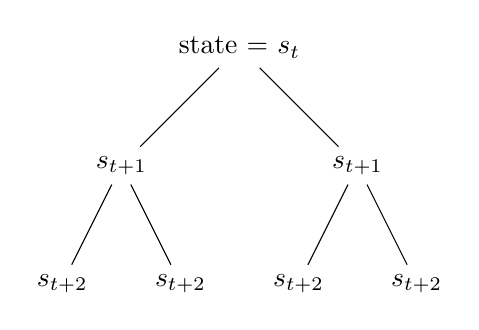
\begin{tikzpicture}[level distance=1.5cm,%
      level 1/.style={sibling distance=3cm},%
      level 2/.style={sibling distance=1.5cm}]%
      \node {state = $s_t$}%
        child {node {$s_{t+1}$}%
          child {node {$s_{t+2}$}}%
          child {node {$s_{t+2}$}}%
        }%
        child {node {$s_{t+1}$}%
        child {node {$s_{t+2}$}}%
          child {node {$s_{t+2}$}}%
        };%
    \end{tikzpicture}%
    \end{center}%
  \end{figure}%
  \begin{itemize}%
    \item[$\blacktriangleright$] \textbf{History state} gives unique path through event tree.%
    \pause%
    \item[$\blacktriangleright$] $s^{t-1}(s^t)$ gives unique predecessor.%
    \pause%
    \item[$\blacktriangleright$] $S^{t+1}(s^t)$ for set of successor or $s^{t+1} \succ s^t$ successor.%
  \end{itemize}%
\end{frame}%
%-------------------------------------------------------------------------
% Making Things Random: Markov Processes (3/3)
\begin{frame}{Making Things Random: Markov Processes (3/3)}%
  We will need to talk about probabilities of different states and events:\\%
  \vspace*{0.2in}%
  \pause%
  \begin{itemize}%
    \item[$\blacktriangleright$] The unconditional probability of a given history state $s^t$ is $Pr\{s^t\}$.%
    \vspace*{0.2in}%
    \pause%
    \item[$\blacktriangleright$] The conditional probability of a history state tomorrow given one today is \[ \frac{ Pr\{s^{t+1}\} }{ Pr\{s^t\}} \] if $s^{t+1} \succ s^t$ and 0 otherwise.%
  \end{itemize}%
\end{frame}%
%-------------------------------------------------------------------------
% BLOCK 2: The Stochastic Cash-in-Advance Model
%-------------------------------------------------------------------------
\section{The Stochastic\\Cash-in-Advance Model\\{\small Cole (2020) chapter 5}}%
%-------------------------------------------------------------------------
% Stochastic CiA Model: Household Setup
\begin{frame}{Stochastic CiA Model: Household Setup}%
  Now, let us introduce Markov chains and state operators into our model! The \textbf{household payoff function} is the discounted probability weighted sum of our flow payoffs:%
  \begin{align*}%
      &\sum_{t=1}^{T} \sum_{s^t} \beta ^{t-1}  \left[ u(C(s^{t}))-v(L(s^{t}))\right] Pr\{s^t\} \\%
      & +\beta ^{T}\sum_{s^{T+1}}V(M(s^{T}),\;B(s^{T}),\;s^{T+1}) Pr\{s^{T+1}\} \\%
      = \; & \mathbb{E} \left\{%
      \begin{array}{c}%
        \sum_{t=1}^T \beta ^{t-1}\left[ u(C(s^{t}))-v(L(s^{t}))\right] \\%
        +\beta ^{T}V(M(s^{T}),\;B(s^{T}),\;s^{T+1})%
      \end{array}%
      \right\}%
    \end{align*}%
  \pause%
  \begin{itemize}%
    \item[$\blacktriangleright$] Our choice variables are: $C(s^t)$, $L(s^t)$, $M(s^t)$, $B(s^t)$.%
    \item[$\blacktriangleright$] We inherit our past choices: $M(s^{t-1}(s^t))$, $B(s^{t-1}(s^t))$.%
    \item[$\blacktriangleright$] We face prices: $P(s^t)$, $q(s^t)$.%
  \end{itemize}%
\end{frame}%
%-------------------------------------------------------------------------
% Stochastic CiA Model: Lagrangian
\begin{frame}{Stochastic CiA Model: Lagrangian}%
  The \textbf{Lagrangian} for this problem is kind of similar to what we had before:%
  \begin{eqnarray*}%
  \mathcal{L} &\mathcal{=}&\max_{\left\{L(s^{t}),\;C(s^{t}),\;M(s^{t}),\;B(s^{t})\right\} _{t=1}^{T}}\min_{\left\{ \mu(s^{t}),\;\lambda (s^{t})\right\} _{t=1}^{T}} \\%
  &&\mathbb{E}\left\{%
  \begin{array}{c}%
    \sum_{t=1}^T \beta ^{t-1}\left[ u(C(s^{t}))-v(L(s^{t}))\right] \\%
    +\beta ^{T}V(M(s^{T}),\;B(s^{T}),\;s_{T+1})%
  \end{array}%
  \right\} \\%
    &&+\sum_{t=1}^T\sum_{s^{t}}\lambda (s^{t})\left\{M(s^{t-1}(s^{t}))-P(s^{t})C(s^{t})\right\} \\%
    &&+\sum_{t=1}^T\sum_{s^{t}}\mu (s^{t})\left\{%
  \begin{array}{c}%
    P(s^{t})Z(s^{t})L(s^{t})+\left[ M(s^{t-1}(s^{t}))-P(s^{t})C(s^{t})\right] \\%
    +B(s^{t-1}(s^{t}))+T(s^{t})-M(s^{t})-q(s^{t})B(s^{t})%%
  \end{array}%
  \right\}.%
  \end{eqnarray*}%
  \pause%
  \begin{itemize}%
    \item[$\blacktriangleright$] $\mathbb{E}$ is the expectation operator representing the weighted average over all states, $\sum_{s^t}$.%
    \item[$\blacktriangleright$] We have a CiA constraint and budget constraint for each history state, $s^t$.%
    \pause%
    \item[$\blacktriangleright$] We have separate multipliers for each history state since they bind differentially.%
  \end{itemize}%
\end{frame}%
%-------------------------------------------------------------------------
% Stochastic CiA Model: First-Order Conditions
\begin{frame}{Stochastic CiA Model: First-Order Conditions}%
  The \textbf{FOCs of the stochastic CiA model} are as follows:%
  \begin{align}%
    \mathcal{L}_{C(s^t)}: & \quad \beta ^{t-1}u^{\prime }(C_t(s^{t}))\Pr (s^{t})-\left[ \lambda (s^{t})+\mu(s^{t})\right] P(s^{t}) \; \overset{!}{=} \; 0\\%
    \notag \\%
    \mathcal{L}_{L(s^t)}: & \quad -\beta ^{t-1}v^{\prime }(L_t(s^{t}))\Pr (s^{t})+\mu (s^{t})P(s^{t})Z(s^{t}) \; \overset{!}{=} \; 0\\%
    \notag \\%
    \mathcal{L}_{M(s^t)}: & \quad -\mu (s^{t})+\sum_{s^{t+1}\in S^{t+1}(s^{t})}\left[ \lambda (s^{t+1})+\mu(s^{t+1})\right] \; \overset{!}{=} \; 0\\%
    \notag \\%
    \mathcal{L}_{B(s^t)}: & \quad -\mu (s^{t})q(s^{t})+\sum_{s^{t+1}\in S^{t+1}(s^{t})}\mu (s^{t+1}) \; \overset{!}{=} \;0%
  \end{align}%
  \begin{itemize}%
    \item[$\rightarrow$] Because the impact of increasing money or bond stocks impacts all successor nodes, we get a summation term.%
  \end{itemize}%
\end{frame}%
%-------------------------------------------------------------------------
% Stochastic CiA Model: Determining the Equilibrium
\begin{frame}{Stochastic CiA Model: Determining the Equilibrium}%
  The steps here are the same: (1) impose market clearing + (2) cash-in-advance constraint:%
  \vspace*{0.15in}%
  \pause%
  \begin{itemize}%
    \item[$\blacktriangleright$] \textbf{Resource constraint:} $C_t = Z_t L_t$%
    \vspace*{0.15in}%
    \item[$\blacktriangleright$] \textbf{Money market clearing:} $M_t = \bar M_t$%
    \vspace*{0.15in}%
    \item[$\blacktriangleright$] \textbf{Binding CiA constraint:}%
    \begin{equation}%
      \implies P(s^{t})=\frac{\bar{M}(s^{t-1}(s^{t}))}{Z(s^{t})L(s^{t})}.%
      \label{price level 1}%
    \end{equation}%
    \vspace*{0.15in}%
    \pause%
    \item[$\blacktriangleright$] Set the preference assumptions as before:%
    \begin{align*}%
      u(C(s^t)) \; = & \; log(C(s^t))\\%
      v(L(s^t)) \; = & \; \frac{L(s^t)^{1+\nu}}{1+\nu}%
    \end{align*}%
  \end{itemize}%  
\end{frame}%
%-------------------------------------------------------------------------
% Stochastic CiA Model: Change-in-Variables
\begin{frame}{Stochastic CiA Model: Change-in-Variables (1/3)}%
  Impose a \textbf{change-in-variables} to render the model stationary! Start with the non-stationary consumption FOC (\emph{log-utility} produces constant adjusted penalty prices across time):%
  \begin{align*}%
    \beta^{t-1}\Pr (s^{t}) \; = & \; \left[ \lambda (s^{t})+\mu(s^{t})\right] P(s^t) C(s^t)\\%
     = & \; \left[ \lambda (s^{t})+\mu(s^{t})\right] \bar M(s^{t-1}(s^t))\\%
     \pause%
    \Leftrightarrow \quad \frac{\beta^{t-1} Pr(s^t)}{M(s^{t-1}(s^t))} \; = & \; \left[ \lambda (s^{t})+\mu(s^{t})\right]%
  \end{align*}\\%
  \vspace*{0.15in}%
  \pause%
  We \textbf{render all penalty prices stationary} by applying the following transformation implied by the above condition:%
  \begin{align*}
    \mu (s^{t}) \; = & \; \frac{\beta ^{t-1}\tilde{\mu}(s^{t})\Pr (s^{t})}{\bar{M}(s^{t-1}(s^{t}))},\\%
    \lambda (s^{t}) \; = & \; \frac{\beta ^{t-1}\tilde{\lambda}(s^{t})\Pr (s^{t})}{\bar{M}(s^{t-1}(s^{t}))}.%
  \end{align*}%
\end{frame}%
%-------------------------------------------------------------------------
% Stochastic CiA Model: Change-in-Variables (2/3)
\begin{frame}{Stochastic CiA Model: Change-in-Variables (2/3)}%
  Using this change-in-variables, \textbf{rewrite our FOCs} as:%
  \begin{align}%
    1 \; = & \; \left[ \tilde{\lambda}(s^{t}) + \tilde{\mu}(s^{t}) \right]\\%
    \notag \\%
    \pause%
    L(s^{t})^{\gamma} \; = & \; \tilde{\mu}(s^{t}) \left[ \frac{1}{L(s^{t})} \right]\\%
    \notag \\%
    \pause%
    \tilde{\mu}(s^{t}) \; = & \; \frac{\beta}{(1+\tau(s^{t}))} \sum_{s^{t+1}\in S^{t+1}(s^{t})} \underbrace{\left[ \tilde{\mu}(s^{t+1})+\tilde{\lambda}(s^{t+1})\right]}_{=1} \frac{Pr(s^{t+1})}{Pr(s^{t})}\\%
    \notag \\%
    \pause%
     q(s^{t}) \; = & \; \frac{\beta}{(1+\tau(s^{t}))} \sum_{s^{t+1}\in S^{t+1}(s^{t})} \frac{\tilde{\mu}(s^{t+1})}{\tilde{\mu}(s^{t})} \frac{Pr(s^{t+1})}{Pr(s^{t})}%
  \end{align}%
\end{frame}%
%-------------------------------------------------------------------------
% Stochastic CiA Model: Change-in-Variables (3/3)
\begin{frame}{Stochastic CiA Model: Change-in-Variables (3/3)}%
  Using this change-in-variables, \textbf{further rewrite our FOCs} as:%
  \begin{align}%
    1 \; = & \; \left[ \tilde{\lambda}(s^{t})+\tilde{\mu}(s^{t})\right]\\%
    L(s^{t})^{\gamma} \; = & \; \tilde{\mu}(s^{t})\left[ \frac{1}{L(s^{t})}\right]\\%
    \tilde{\mu}(s^{t}) \; = & \; \frac{\beta}{(1+\tau(s^{t}))}\label{eq:foc_money}\\%
    q(s^t) \; = & \; \sum_{s^{t+1}\in S^{t+1}(s^{t})} \frac{\beta}{(1+\tau(s^{t+1}))}\Pr(s_{t+1}|s_t)%
  \end{align}%
  \pause%
  \begin{itemize}%
    \item[$\blacktriangleright$] $q_t$ is simply the real discount rate times the expected component of inflation coming from the expected increase in the money supply.%
    \pause%
    \item[$\blacktriangleright$] Nothing in these equations reflects the past, and hence \textbf{everything is a function of the current state $s_t$ only.}%
  \end{itemize}%
\end{frame}%
%-------------------------------------------------------------------------
% Stochastic CiA Model: Forecasting the Future and Bond Prices
\begin{frame}{Stochastic CiA Model: Forecasting the Future and Bond Prices}%
  \begin{itemize}%
    \item[$\blacktriangleright$] In the bond price equation,%
    \begin{align*}%
      q(s_t) \; = & \; \sum_{s_{t+1}} \frac{\beta}{(1+\tau(s_{t+1}))}\Pr(s_{t+1}|s_t)%
    \end{align*}%
    we are trying to forecast next period's growth rate from the current state.%
    \pause%
    \item[$\blacktriangleright$] Really this is all about%
    \begin{align*}%
      \sum_{\tau_{t+1}} \frac{1}{1+\tau(s_{t+1})} Pr\{ \tau_{t+1} | \tau_t, g_t\}.%
    \end{align*}%
    \pause%
    \item[$\blacktriangleright$] The $g_t$ terms comes in just if there is any correlation between the two.%
    \begin{itemize}%
      \begin{small}%
        \item[$\rightarrow$] Note: $1/ E \{x\} \neq E \{1/x\}$ {\footnotesize (Jensen's inequality)}.%
      \end{small}%
    \end{itemize}%
    \pause%
    \item[$\blacktriangleright$] The labor equation is just analytic, so this one is going to be easy%
    \begin{align*}%
      L_t \; = \; \left[ \frac{\beta}{(1 + \tau_t)} \right]^{1/(1+\gamma)}.%
    \end{align*}%
  \end{itemize}%
\end{frame}%
%-------------------------------------------------------------------------
% Approach to Compute the Stochastic CiA Model
\begin{frame}{Approach to Compute the Stochastic CiA Model}%
  We take \textbf{two approaches to adding in stochastic shocks} and computing equilibria:%
  \vspace*{0.1in}%
  \pause%
  \begin{enumerate}%
    \item Use simple Markov chains which consist of a small set of possible realizations.%
    \pause%
    \item Use standard first-order autoregressive (AR(1)) processes with normal shocks.%
  \end{enumerate}%
  \vspace*{0.2in}%
  \pause%
  In both cases, we will calibrate the shock processes, draw some shocks and use them to simulate our model.%
\end{frame}%
%-------------------------------------------------------------------------
% BLOCK: Stochastic Computer Model with Markov Chains
%-------------------------------------------------------------------------
\section{Stochastic Computer Model with Markov Chains\\{\small Cole (2020) chapter 5}}%
%-------------------------------------------------------------------------
% Markov Chains: Transition and Probabilities (1/2)
\begin{frame}{Markov Chains: Transition and Probabilities (1/2)}%
  Assume that ...%
  \begin{itemize}%
    \item[$\blacktriangleright$] our random variable $x$ can only take on a discrete set of values: $x \in X = \{x_1,...,x_n\}$.%
    \item[$\blacktriangleright$] the probability of going from $x_i$ this period to $x_j$ next period is simply given by $Q(i,j)$.%
    \begin{itemize}%
      \item[$\rightarrow$] Note: $\sum_{j=1}^{n} Q(i,j) = 1$ since this exhausts the possibilities.%
    \end{itemize}%
  \end{itemize}%
  \pause%
  We summarize all transition probabilities in a \textbf{transition matrix $\mathbb{Q}$:}%
  \begin{itemize}%
    \item[$\blacktriangleright$] The row number says where you are today.%
    \item[$\blacktriangleright$] The column number is where you might go tomorrow.%
    \pause%
    \item[$\blacktriangleright$] For example $x \in \{1,2,3\}$ where $x_1 > x_2 > x_3$. and \[ \mathbb{Q} = \left [ \begin{array}{ccc} .3 & .4 & .3 \\ .2 & .45 & .35 \\ .1 & .5 & .4 \end{array} \right ] \]%
    \begin{itemize}%
      \item[$\rightarrow$] the first row gives the transition probabilities if today is $i$.%
      \item[$\rightarrow$] and the columns are for going to $1, 2, 3$ respectively.%
    \end{itemize}%
  \end{itemize}%
\end{frame}%
%-------------------------------------------------------------------------
% Markov Chains: Transition and Probabilities (2/2)
\begin{frame}{Markov Chains: Transition and Probabilities (2/2)}%
  Let there be a vector of the \textbf{probabilities of being in each state} $X$ at time $t$:\\%
  \[ \mathbb{P}_t = \left [ \begin{array}{c} p_1 \\ p_2 \\ p_3 \end{array} \right ]^T \]%
  \pause%
  It follows that:%
  \begin{itemize}%
    \item[$\blacktriangleright$] The probability of being in each state next period is given by: $\mathbb{P}_{t+1} =  \mathbb{P}_t \mathbb{Q}$%
    \vspace*{0.05in}%
    \item[$\blacktriangleright$] This means that: $p_{t+1}(j) = \sum_i p_{t}(i) Q(i,j)$%
    \vspace*{0.05in}%
    \pause%
    \item[$\blacktriangleright$] The \emph{probability $n$-steps ahead} is given by: $\mathbb{P}_{t+n} =  \mathbb{P}_t \mathbb{Q}^n$%
    \vspace*{0.05in}%
    \pause%
    \item[$\blacktriangleright$] A \emph{stationary distribution} is such that: $\mathbb{P} =  \mathbb{P} \mathbb{Q}$%
    \vspace*{0.05in}%
    \pause%
    \item[$\blacktriangleright$] If $Q(i,j)>0 \; \forall i,j$, then $\mathbb{Q}$ has a unique stationary distribution and for any $\mathbb{P}_0$ it follows: $$\mathbb{P} = lim_{n \rightarrow \infty} \mathbb{P}_0 \mathbb{Q}^n$$%
  \end{itemize}%
\end{frame}%
%-------------------------------------------------------------------------
% Markov Chains: Defining the Productivity Growth Rate Process
\begin{frame}{Markov Chains: Defining the Productivity Growth Rate Process}%
  Let us \textbf{calibrate our Markov processes.} Assume that ...%
  \pause%
  \begin{itemize}%
    \item[$\blacktriangleright$] the productivity growth rate shock has mean $0.03$ and variance $0.002$ (approx. US data).%
    \item[$\blacktriangleright$] productivity growth rates are i.i.d.%
    \item[$\blacktriangleright$] we want a two-state symmetric Markov chain with the above properties.%
  \end{itemize}%
  \pause%
  It follows that ...%
  \begin{itemize}%
    \item[$\blacktriangleright$] High growth rate, $g_h = 0.03+a$, and low growth rate, $g_l = 0.03-a$.%
    \item[$\blacktriangleright$] Transition matrix: $\mathbb{Q} = \left [ \begin{array}{cc} .5 & .5 \\ .5 & .5  \end{array} \right ]$%
    \item[$\blacktriangleright$] Unique stationary distribution (due to symmetry) is $\mathbb{P} = [0.5, 0.5]$.%
  \end{itemize}%
  \pause%
  We can check the process by calculating the variance of g:%
  \begin{gather*} 0.5 [g_h - 0.03 ] ^2 + 0.5 [g_l - 0.03]^2 = a^2 = 0.002 \\%
    \implies a = 0.002^{0.5} = 0.05%
  \end{gather*}\\%
  \vspace*{-0.2in}%
\end{frame}%
%-------------------------------------------------------------------------
% Markov Chains: Defining the Money Growth Rate Process
\begin{frame}{Markov Chains: Defining the Money Growth Rate Process}%
  Next, \textbf{calibrate} inflation over the long haul, which is given by $\frac{1 + \tau} {1 + g}$. Assume that ...%
  \begin{itemize}%
    \item[$\blacktriangleright$] It is roughly $2$ percent on average.%
    \item[$\blacktriangleright$] It tends to be fairly persistent. So, let's assume $ \mathbb{Q} = \left [ \begin{array}{cc} .75 & .25 \\ .25 & .75  \end{array} \right ] $.%
    \item[$\blacktriangleright$] The unique stationary distribution (due to symmetry) is still $\mathbb{P} = [0.5,0.5]$%
    \item[$\blacktriangleright$] The mean of $\tau$ is $5$ percent.%
    \item[$\blacktriangleright$] Assume the variance is the same as $g$.% 
  \end{itemize}%
  \pause%
  It follows that ...%
  \begin{itemize}%
    \item[$\blacktriangleright$] High growth rate: $\tau_h = 0.05+a$%
    \item[$\blacktriangleright$] Low growth rate: $\tau_l = 0.05-a$%
    \item[$\blacktriangleright$] Standard deviation: $a = 0.05$%
  \end{itemize}%
  \vspace*{0.2in}%
  \pause%
  \begin{center}%
    \textbf{Now we are ready to try and put this on the computer.}%
  \end{center}%
\end{frame}%
%-------------------------------------------------------------------------
% Markov Chains: Creating Shocks and Outcomes (1/2)
\begin{frame}{Markov Chains: Creating Shocks and Outcomes (1/2)}%
  Generate a sequence of outcomes for random variables $\{g,\tau\}$ using the transition matrix.%
  \begin{small}%
    \begin{enumerate}%
      \item Draw a uniform random variable:%
      \begin{itemize}%
        \item[$\rightarrow$] Go to state 0 if $x < Q(i,0)$.%
        \item[$\rightarrow$] Otherwise go to state 1, where $i$ is the current state.%
      \end{itemize}%
      \vspace*{0.1in}%
      \pause%
      \item Given draws of $\{\tau_t\}$ compute the labor supply:%
      \begin{align*}%
        L(\tau_t) \; = \; \left[ \frac{\beta}{1+\tau_t} \right]^{1/(1+\gamma)}%
      \end{align*}%
      \pause%
      \item Compute the growth rate of output and prices, having already determined labor:%
      \begin{align*}%
        \frac{Y_t}{Y_{t-1}} \; = & \; (1+g_t)\frac{L_t}{L_{t-1}}\\%
        \frac{P_t}{P_{t-1}} \; = & \; \frac{1+\tau_t}{1+g_t} \frac{L_{t-1}}{L_{t}}%
      \end{align*}%
      \pause%
      \item Note that changes in relative labor will affect the volatility of the growth rates. We might want to revisit our calibration in light of this.%
    \end{enumerate}%  
  \end{small}%
\end{frame}%
%-------------------------------------------------------------------------
% Markov Chains: Creating Shocks and Outcomes (2/2)
\begin{frame}{Markov Chains: Creating Shocks and Outcomes (2/2)}%
  \begin{small}%
    \begin{enumerate}%
      \item[6.] All that is left is the bond price, remember that%
      \begin{align*}%
        q(s_t) \; = \; \sum_{\tau_{t+1}} \frac{1}{1+\tau_{t+1}} Pr\{ \tau_{t+1} | \tau_t, g_t\}%
      \end{align*}%
      \pause%
      \item[7.] Conditional expectation of the growth rate of money at $t+1$ given state at $t$. There are two cases:%
      \pause%
      \begin{itemize}%
        \item[$\rightarrow$] If $\tau = \tau_h$ then \[ \mathbb{E} \left[ \frac{1}{1+\tau_{t+1} } \Big | \tau_h \right] = \frac{0.75}{1+\tau_h} +  \frac{0.25}{1+\tau_l} \]%
        \pause%
        \item[$\rightarrow$] If $\tau = \tau_l$ then \[ \mathbb{E} \left [ \frac{1}{1+\tau_{t+1} } \Big | \tau_l \right ] = \frac{0.25}{1+\tau_h} +  \frac{0.75}{1+\tau_l} \]%
      \end{itemize}%
    \end{enumerate}%
  \end{small}%
\end{frame}%
%-------------------------------------------------------------------------
% BLOCK XX: Stochastic Computer Model with AR(1)-Processes
%-------------------------------------------------------------------------
\section{Stochastic Computer Model with AR(1)-Processes\\{\small Cole (2020) chapter 6}}%
%-------------------------------------------------------------------------
% AR(1)-Process: Basic Setup (1/2)
\begin{frame}{AR(1)-Process: Basic Setup (1/2)}%
  \begin{itemize}%
    \item[$\blacktriangleright$] Our random variables are going to follow simple AR(1) processes in which%
    \begin{align*}%
      x_{t} \; = \; Ax_{t-1}+B+C\varepsilon _{t},%
    \end{align*}%
    \pause%
    \item[$\blacktriangleright$] So long as the expected value of $\varepsilon _{t}=0$,%
    \begin{align*}%
      \mathbb{E} \left\{ x_{t}\right\} \; = \; A E \left\{ x_{t-1}\right\} +B.%
    \end{align*}%
    \pause%
    \item[$\blacktriangleright$] Since this is an unconditional expectation, $\mathbb{E}\left\{%
    x_{t}\right\} = \mathbb{E} \left\{ x_{t-1}\right\},$ hence%
    \begin{align*}%
    \mathbb{E} \left\{ x_{t}\right\} =\frac{B}{1-A},%
    \end{align*}%
  \end{itemize}%
\end{frame}%
%-------------------------------------------------------------------------
% AR(1)-Process: Basic Setup (2/2)
\begin{frame}{AR(1)-Process: Basic Setup (2/2)}%
  \begin{itemize}%
    \item[$\blacktriangleright$] Next, note that we can recursively substitute:%
    \begin{align*}%
      x_{t} \; = & \; B+C\varepsilon _{t}+A\left\{ B+C\varepsilon _{t-1}\right\}+A^{2}\left\{ B+C\varepsilon _{t-2}\right\} +... \\%
      = & \; \frac{B}{1-A}+C\sum_{j=0}^{\infty }A^{j}\varepsilon _{t-j}%
    \end{align*}%
    \pause%
    \item[$\blacktriangleright$] This is because {\footnotesize(geometric series)}: \[ 1 + A + A^2 + A^3 + ... = \frac{1}{1-A} \]%
    \pause%
    \item[$\blacktriangleright$] $A$ is governing how persistent a shock is:%
    \begin{itemize}%
	    \item[$\rightarrow$] First period $C\varepsilon _{t}$%
	    \item[$\rightarrow$] Second period $AC\varepsilon _{t}$%
	    \item[$\rightarrow$] Third period $A^2C\varepsilon _{t}$%
    \end{itemize}%
  \end{itemize}%
\end{frame}%
%-------------------------------------------------------------------------
% AR(1)-Process: Examples
\begin{frame}{AR(1)-Process: Examples}%
  Here we simulate a simple AR(1): $x_t = \rho x_{t-1} + \epsilon_t$ for values of $\rho$.%
  \begin{figure}%
    \begin{subfigure}{0.45\textwidth}%
      \hfill%
      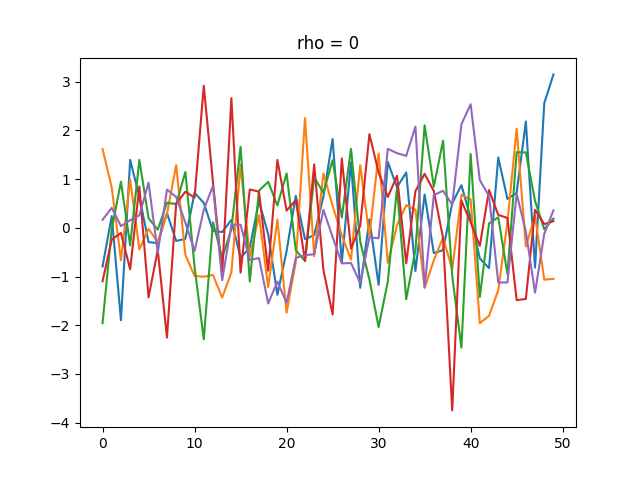
\includegraphics[width=0.7\textwidth]{figures/rand1.png}%
    \end{subfigure}%
    \hfill%
    \begin{subfigure}{0.45\textwidth}%
      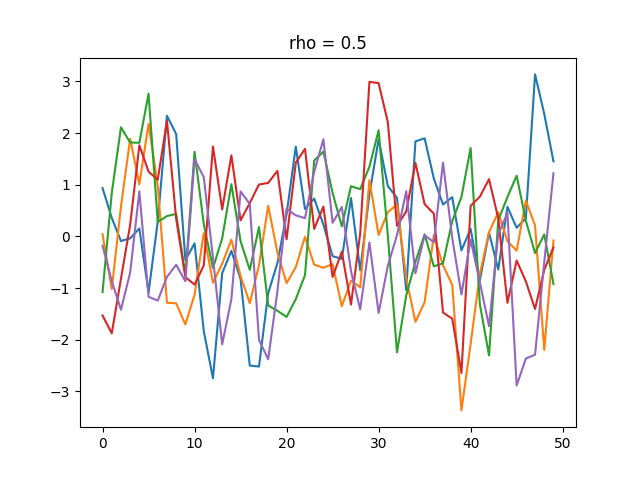
\includegraphics[width=0.7\textwidth]{figures/rand2.png}%
      \hfill%
    \end{subfigure}\\%
    \begin{subfigure}{0.45\textwidth}%
      \hfill%
      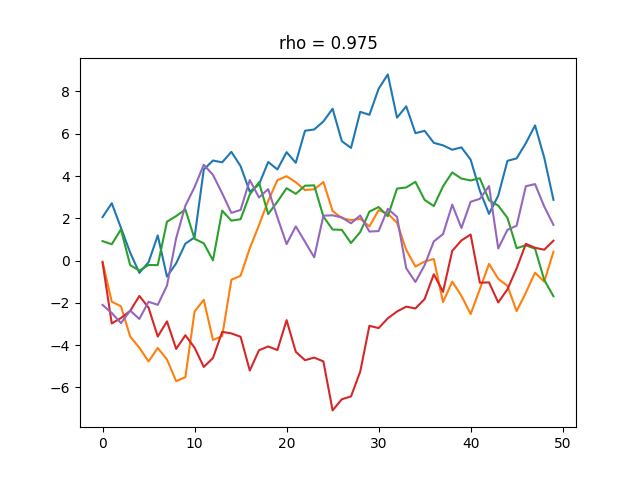
\includegraphics[width=0.7\textwidth]{figures/rand3.png}%
    \end{subfigure}%
    \hfill%
    \begin{subfigure}{0.45\textwidth}%
      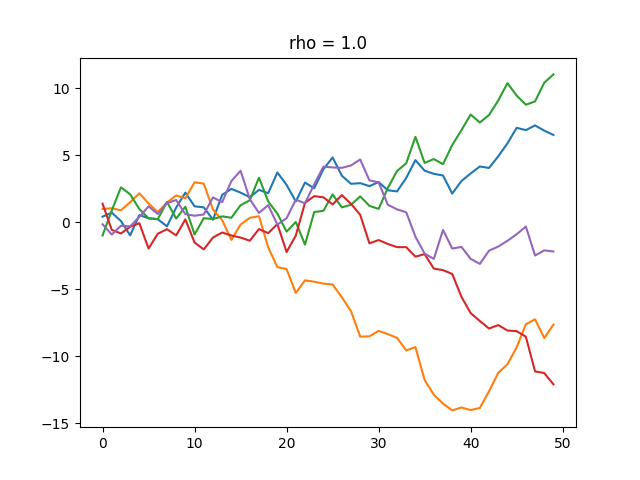
\includegraphics[width=0.7\textwidth]{figures/rand4.png}%
      \hfill%
    \end{subfigure}%
  \end{figure}%
  \pause%
  \begin{center}%
    What happens to the AR(1) process if $\rho>1$?%
  \end{center}%
\end{frame}%
%-------------------------------------------------------------------------
% AR(1)-Process in our Stochastic Model
\begin{frame}{AR(1)-Process in our Stochastic Model}%
  \begin{itemize}%
    \item[$\blacktriangleright$] In our set-up, $x_{t}$ will be a vector:%
    \begin{align*}%
      x_{t}=\left[%
      \begin{array}{c}%
        \tau _{t} \\%
        g_{t}%
      \end{array}%
      \right]%
    \end{align*}%
    \pause%
    \item[$\blacktriangleright$] And our AR(1)-process is:%
    \begin{align*}%
      x_{t}=\left[%
      \begin{array}{cc}%
        \rho _{\tau } & 0 \\%
        0 & \rho _{g}%
      \end{array}%
      \right] x_{t-1}+\left[%
      \begin{array}{c}%
        B_{\tau } \\%
        B_{g}%
      \end{array}%
      \right] +\left[%
      \begin{array}{cc}%
        \sigma _{\tau } & 0 \\%
        0 & \sigma _{g}%
      \end{array}%
      \right] \left[%
      \begin{array}{c}%
        \varepsilon _{\tau ,t} \\% 
        \varepsilon _{g,t}%
      \end{array}%
      \right]%
    \end{align*}%
    \begin{itemize}%
      \item[$\rightarrow$] Zero entries on the off-diagonals indicate that both the process and shocks have no cross-correlations!%
    \end{itemize}%
    \vspace*{0.1in}%
    \pause%
    \item[$\blacktriangleright$] So, the long-run means here is:%
    \begin{align*}%
      \left[%
      \begin{array}{c}%
        B_{\tau}/(1 - \rho_{\tau}) \\%
        B_{g}/(1 - \rho_{g})%
      \end{array}%
      \right]%
    \end{align*}%
  \end{itemize}%
\end{frame}%
%-------------------------------------------------------------------------
% AR(1)-Process: Transition and Probabilities (1/3)
\begin{frame}{AR(1)-Process: Transition and Probabilities (1/3)}%
  In our theory we talk about $Pr\{s_{t+1}|s_t\}$. What does this mean?%
  \begin{itemize}%
    \item[$\blacktriangleright$] Start from our state vector $s_{t}=\left( Z_{t-1},\bar{M}_{t-1},\tau _{t},g_{t}\right).$%
    \pause%
    \item[$\blacktriangleright$] The only state $s_{t+1}$ that can follow must have $Z_{t}=Z_{t-1}(1+g_{t})$ and $\bar{M}_{t}=(1+\tau_{t})\bar{M}_{t-1}:$%
    \begin{itemize}%
      \item[$\rightarrow$] Either probability $0$.%
      \item[$\rightarrow$] Or $s_{t+1} = ( Z_{t-1}(1+g_{t}),(1+\tau_{t})\bar{M}_{t-1} ,\tau_{t+1},g_{t+1})$.%
    \end{itemize}%
    \pause%
    \item[$\blacktriangleright$] However, there is a wide range of possible values for $\tau _{t+1} $ and $g_{t+1}$. We need to put probabilities on these possible outcomes.%
    \pause%
    \item[$\blacktriangleright$] Once we do, the probability of \[ s_{t+1} = ( Z_{t-1}(1+g_{t}),(1+\tau_{t})\bar{M}_{t-1} ,\tau _{t+1},g_{t+1}) \] is simply \[ Pr\{s_{t+1}|s_t\} = Pr\{\tau _{t+1},g_{t+1} | \tau _{t},g_{t}\} \]%
  \end{itemize}%
\end{frame}%
%-------------------------------------------------------------------------
% AR(1)-Process: Transition and Probabilities (2/3)
\begin{frame}{AR(1)-Process: Transition and Probabilities (2/3)}%
  \begin{itemize}%
    \item[$\blacktriangleright$] For a given $\tau _{t+1}$ to follow from $\tau _{t},$ it must be the case that the realized shock satisfies:
    \begin{align*}%
      \tau_{t+1} \; = \; \rho_{\tau}\tau_{t}+B_{\tau}+\sigma_{\tau}\varepsilon_{\tau,t+1}%
    \end{align*}%
    \vspace*{-0.2in}%
    \begin{itemize}%
      \item[$\rightarrow$] Hence, there is a unique shock associated with this realization.%
    \end{itemize}%
    \vspace*{0.2in}%
    \pause%
    \item[$\blacktriangleright$] Denote the probability of that shock as:%
    \begin{align*}%
      \Pr (\varepsilon_{\tau, t+1}) \; = \; \Pr \left( \frac{\tau_{t+1}-\rho_{\tau }\tau_{t}-B_{\tau }}{\sigma_{\tau}}\right)%
    \end{align*}%
    \pause%
    \item[$\blacktriangleright$] Similarly if $g_{t+1}$ is the realized growth rate, then the associated shock must satisfy: \[g_{t+1}=\rho _{g}g_{t}+B_{g}+\sigma _{g}\varepsilon _{g,t+1}\] and hence the probability of that realization is: \[\Pr \left( \varepsilon _{g,t+1}\right) =\Pr \left( \frac{g_{t+1}-\rho_{g}g_{t}-B_{g}}{\sigma _{g}}\right) \]%
  \end{itemize}%
\end{frame}%
%-------------------------------------------------------------------------
% AR(1)-Process: Transition and Probabilities (3/3)
\begin{frame}{AR(1)-Process: Transition and Probabilities (3/3)}%
  \begin{itemize}%
    \item[$\blacktriangleright$] Thus, the conditional probability of going from \[ s_{t}=\left( Z_{t-1},\bar{M}_{t-1},\tau _{t},g_{t}\right) \] to \[ s_{t+1}=\left( Z_{t-1}(1+g_{t}),(1+\tau _{t})\bar{M}_{t-1},\tau_{t+1},g_{t+1}\right) \] is given by: \[ \Pr \left( s_{t+1}|s_{t}\right) =\Pr \left( \frac{\tau _{t+1}-\rho _{\tau}\tau _{t}-B_{\tau }}{\sigma _{\tau }}\right) \Pr \left( \frac{g_{t+1}-\rho_{g}g_{t}-B_{g}}{\sigma _{g}}\right) .\]%
    \begin{itemize}%
      \item[$\rightarrow$] This last bit follows from our independence assumption for our two shocks.%
    \end{itemize}%
  \end{itemize}%
\end{frame}%
%-------------------------------------------------------------------------
% AR(1)-Process: Reduced Form Model
\begin{frame}{AR(1)-Process: Reduced Form Model}%
  Our economy can be boiled down to two key equations.%
  \pause%
  \begin{enumerate}%
    \item The first is our labor supply condition:%
    \begin{align}%
      L(s_{t}) \; = & \; \left[ \frac{\beta}{(1+\tau_{t}(s^{t}))} \right]^{\frac{1}{1+\gamma}} \label{D1}%
    \end{align}%
    \pause%
    \item The second equation is our interest rate condition:%
    \begin{align}%
      q(s_{t}) \; = & \; \sum_{s^{t+1}\in S^{t+1}(s^{t})}\left[ \frac{\beta }{(1+\tau_{t+1}(s^{t+1}))}\right] \Pr (s_{t+1}|s_{t}).%
    \end{align}%
    \begin{itemize}%
      \item[$\rightarrow$] Approximating an integral can be done in clever ways, but we are not going to bother.%
      \pause%
      \item[$\rightarrow$] Instead, we draw enough $\varepsilon_{t+1}$ shocks using a random number generator to get a representative distribution and use them in an approximation. So draw $\mathbb{C} = \{\varepsilon_1, ..., \varepsilon_N \}$.%
      \pause%
      \item[$\rightarrow$] Then just compute the implied update for each shock and take the appropriate mean \[ \mathbb{E} \left [ \frac{1}{1+\tau_{t+1}} \Big | \tau_t \right ] = \frac{1}{N} \sum_{i=1}^N \left[ \frac{1}{1+\rho _{\tau }\tau _{t}+B_{\tau }+\sigma _{\tau }\varepsilon_{i} } \right] \].%
    \end{itemize}%
  \end{enumerate}%
\end{frame}%
%-------------------------------------------------------------------------
% Calculating Model Statistics
%-------------------------------------------------------------------------
\section{Calculating Model Statistics\\{\small Cole (2020) chapter 6}}%
%-------------------------------------------------------------------------
% Constructing Non-Stationary Variables
\begin{frame}{Constructing Non-Stationary Variables}%
  We've focused on the stationary random variables implied by our model. We can construct the nonstationary one too.%
  \pause%
  \begin{itemize}%
    \item[$\blacktriangleright$] We can construct the money supply recursively using the fact that%
    \begin{align*}%
      M_{t} \; = \; M_{t-1}\left(1+\tau _{t}\right)%
    \end{align*}%
    where we take $M_{0}=1$.%
    \medskip%
    \pause%
    \item[$\blacktriangleright$] We can do the same thing for productivity, $Z_{t}$:%
    \begin{align*}%
      Z_t \; = \; Z_{t-1} \left(1 + g_t\right)%
    \end{align*}%%
    where we take $Z_{0}=1$.%
  \end{itemize}%
\end{frame}%
%-------------------------------------------------------------------------
% Calculating Growth Rates of the Variables
\begin{frame}{Calculating Growth Rates of the Variables}%
  \begin{itemize}%
    \item[$\blacktriangleright$] Consumption is given by:%
    \begin{align*}%
      C_{t}=Z_{t}L_{t}%
    \end{align*}%
    \item[$\blacktriangleright$] The price level is given by:%
    \begin{align*}%
      P_{t}=\frac{M_{t-1}}{Z_{t}L_{t}}%
    \end{align*}%
  \end{itemize}%
  \bigskip%
  \pause%
  With \textbf{nonstationary series} it is common to view them in growth rates:%
  \begin{itemize}%
    \item[$\blacktriangleright$] So if we have output $Y_t$ and it grows at rate $1+g_t$ then:
    \begin{align*}%
      \frac{Y_t}{Y_{t-1}} \; = \; \frac{Y_{t-1}(1+g_t)}{Y_{t-1}}  = 1+g_t%
    \end{align*}%
    \item[$\blacktriangleright$] Similarly, we can construct the inflation rate series as:
    \begin{align*}%
      \frac{P_t}{P_{t-1}} \; = \; 1+\pi_t%
    \end{align*}%
  \end{itemize}%
\end{frame}%
%-------------------------------------------------------------------------
% Calculating Growth Statistics
\begin{frame}{Calculating Growth Statistics}%
  By calculating statistics about our growth processes, we can ...%
  \begin{small}%
    \begin{itemize}%
      \item[$\blacktriangleright$] ask what is the mean growth rate:%
      \begin{align*}%
        \bar g \; = \; \frac{1}{N} \sum_{t=1}^N g_t%
      \end{align*}%
      \pause%
      \item[$\blacktriangleright$] ask what is the variance of our growth rate:%
      \begin{align*}%
        var(g) \; = \; \frac{1}{N} \sum_{t=1}^N (g_t - \bar g)^2
      \end{align*}%
      \pause%
      \item[$\blacktriangleright$] ask if output and inflation are correlated by computing:%
      \begin{align*}%
        corr(g,\pi) \; = \; \frac{ \frac{1}{N} \sum_{t=1}^N (g_t - \bar g)(\pi_t - \bar \pi) }{\sqrt{var(g)var(\pi)}}%
      \end{align*}%
      \pause%
      \item[$\blacktriangleright$] Matlab has a bunch of statistical tools we can use like \emph{mean}, \emph{max}, \emph{median}, \emph{std}, and \emph{corrcoef}.%
    \end{itemize}%
  \end{small}%
\end{frame}%
%-------------------------------------------------------------------------
% Using Growth Statistics: Inflation and Output
\begin{frame}{Using Growth Statistics: Inflation and Output}%
  \begin{block}{Example}%
    We can ask if systematic inflation is correlated with systematic growth in output?%
  \end{block}%
  \medskip%
  \pause%
  \textbf{Procedure:}%
  \begin{small}%
    \begin{enumerate}%
      \item Compute the average growth rate over some interval of time, e.g.:%
      \begin{align*}%
        (1+G_t) \; = & \; \left (\frac{Y_t}{Y_{t-3}} \right )^{1/3} = \left ((1+g_t) (1+g_{t-1})(1+g_{t-2}) \right )^{1/3} \\%
        (1+ \Pi_t) \; = & \; \left (\frac{P_t}{P_{t-3}} \right )^{1/3} = \left ((1+\pi_t) (1+\pi_{t-1})(1+\pi_{t-2}) \right )^{1/3}%
      \end{align*}%
      \begin{itemize}%
        \item[$\rightarrow$] This will give us the average growth rate of that interval.%
      \end{itemize}%
      \pause%
      \item Compute these average growth rates at each point in time $t$.%
      \pause%
      \item Check if these averages $1+G_t$ and $1 + \Pi_t$ are correlated.%
    \end{enumerate}%
  \end{small}%
\end{frame}%
%-------------------------------------------------------------------------
% Sample Statistics vs. Analytical Statistics
\begin{frame}{Sample Statistics vs. Analytical Statistics}%
  We regularly compute all kinds of statistics in the data and from our models:%
  \begin{itemize}%
    \item[$\blacktriangleright$] How seriously should we take them?%
    \item[$\blacktriangleright$] Will they change a lot if we just wait for some more data to come in?%
  \end{itemize}%
  \pause%
  One way to examine this is to \textbf{analytically derive the distribution} of our statistics.%
  \begin{itemize}%
    \item[$\blacktriangleright$] For example: If we have a sample of size $n$ of normal random variables with mean $\mu$ and standard deviation $\sigma$, then ...%
    \begin{small}%
      \begin{itemize}%
        \item[$\rightarrow$] the sample mean has expected value \[ \mathbb{E} \bar X = E n^{-1} \sum_{t=1}^{n} X_t = \mu \]%
        \item[$\rightarrow$] and variance \[ \mathbb{E} ( \bar X - \mu)^2 = E \left [ n^{-1} \sum_{t=1}^{n} X_t - \mu \right ]^2  = E \left [ n^{-2} \sum_{t=1}^{n} (X_t - \mu)^2  \right ] = \frac{\sigma^2}{n} \]%
      \end{itemize}%
    \end{small}%
    \pause%
    \item[$\blacktriangleright$] This gives us an analytic expression for how accurate our sample mean is, given our sample size and the variance of the random variable.%
    \item[$\blacktriangleright$] \textbf{But in general this is hard to do!}%
  \end{itemize}%
\end{frame}%
%-------------------------------------------------------------------------
% Calculating Distributions: Monte Carlo Simulations
\begin{frame}{Calculating Distributions: Monte Carlo Simulations}%
  \begin{itemize}%
    \item[$\blacktriangleright$] An easy thing to do is to examine the distribution of a statistic in our model.\\Standard approach: \textbf{Monte Carlo simulation!}%
    \pause%
    \begin{enumerate}%
      \item Draw different sequences of the shocks indexed by $i$, $\{ \epsilon^{i}_{t} \}$.%
      \pause%
      \item Build up the implied outcomes for each sequence.%
      \pause%
      \item Compute the sample statistic for each sequence $i$, which we can denote by $m_i$.
      \pause%
      \item Examine the distribution of this sample statistic.%
    \end{enumerate}%
    \medskip%
    \pause%
    \item[$\blacktriangleright$] This distribution gives us a lot of information about the accuracy of our estimate and is suggestive as to the accuracy of the data estimate as well.%
    \pause%
    \begin{itemize}%
      \item[$\rightarrow$] One way to think about accuracy is the standard deviation of $m_i$ just as in our example with the sample mean of the normally distributed random variable.%
      \pause%
      \item[$\rightarrow$] A more fundamental way to examine $m_i$ is to plot the histogram. From this plot we can determine a $95 \%$ confidence interval for our model-based statistic.%
    \end{itemize}%
  \end{itemize}%
\end{frame}%
%-------------------------------------------------------------------------
% Conclusions
%-------------------------------------------------------------------------
\section{Conclusions}%
%-------------------------------------------------------------------------
% Summarizing the Lecture
\begin{frame}{Summarizing the Lecture}%
  \begin{center}%
    \begin{large}%
      Can you summarize the three main aspects of the lecture?%
    \end{large}%
  \end{center}%
\end{frame}%
%-------------------------------------------------------------------------
% Concluding Remarks
\begin{frame}{Concluding Remarks}%
  \begin{block}{Big Picture of the Lecture:}%
    \begin{enumerate}%
      \item How do random processes impact the results of the CiA model economy?%
      \item What role do expectations play in our CiA model?%
      \item How can we compare model statistics with the data?%
    \end{enumerate}%
  \end{block}%
  \vspace*{0.1in}%
  \pause%
  \begin{itemize}%
    \item[$\blacktriangleright$] A stochastic model with \textbf{Markov processes:}%
    \begin{itemize}%
      \item[$\rightarrow$] The probability of future states can be described by the current state.%
      \item[$\rightarrow$] Expectations can be formed by weighting future states with their probability.%
      \item[$\rightarrow$] Otherwise, the model shows the same equations as before. Solutions can be easily derived.%
    \end{itemize}%
    \pause%
    \item[$\blacktriangleright$] A stochastic model with \textbf{AR(1) processes:}%
    \begin{itemize}%
      \item[$\rightarrow$] A growth process depends on its realization in the previous period and a random shock.%
      \item[$\rightarrow$] Any AR(1) process can be transformed into a Markov process.%
      \item[$\rightarrow$] Any calculation of the AR(1) model is symmetric to the Markov model.%
    \end{itemize}%
    \pause%
    \item[$\blacktriangleright$] Identifying \textbf{model statistics:}%
    \begin{itemize}
      \item[$\rightarrow$] This allows to compare the model to the data!%
    \end{itemize}
  \end{itemize}%
\end{frame}%
%-------------------------------------------------------------------------
% References
\begin{frame}{References}%
  \begin{itemize}%
    \item[$\blacktriangleright$] Cochrane, John H. (1988). How big is the random walk in GNP?. Journal of political economy, 96(5), 893-920.%
    \item[$\blacktriangleright$] Cole, Harold L. (2020). Monetary and Fiscal Policy through a DSGE Lens. Oxford University Press.%
  \end{itemize}%
\end{frame}%
%-------------------------------------------------------------------------
\end{document}%